\graphicspath{ {./images/} }

\section{Experiments}
\label{sec:experiments}

\subsection{State machines}
I wanted to create something where you could enter a state, invoke the start function once, and then repeatedly invoke the update function. I tried to do this with structs, but I couldn't get it to work. I ended up using a switch statement to check the state and then execute the corresponding code. I am not sure if this is the best way to tackle this, but it sure is a way that I think works pretty okay and is easily understandable.

\subsection{Interrupts}
I had never worked with interrupts before in embedded systems, so I had to do some research on how to use them. I found a good tutorial that explained how to use them. I used the same method for both the horn and the brake. Eventually, I also got word that I had to use interrupts for the Hall sensor, but sadly I didn't get this to work. I hope to eventually look into the Hall sensor again since it is a useful component.

\subsection{Hall sensor}
I have tried to get the Hall sensor working, but I was not able to get it working. I have tried multiple different ways to get it working, for example:
\begin{itemize}
    \item Interrupts
    \item While loops
    \item GPIO readings
\end{itemize}
Sometimes I ended up with a value between 0-10 which spiked to more than 1000, or I ended up with backtrace errors. Eventually, I just wanted to be done with it so I decided to leave it out for now.

\subsection{Motor}
I was struggling a lot with my motor. All the documentation I could find was for Arduino. Not everywhere did it mention the need for an external power source, and when I thought I had it right, not much happened. I went through three DC motors because they stopped working. I tried to repair one, but unfortunately, it didn't yield any results. 
\\ \\
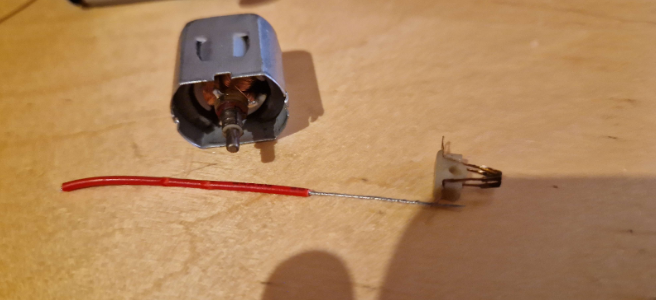
\includegraphics[scale=0.5]{img/motor.png}
\\ \\
Finally, I managed to get the motor running once and adjust the speed with the potentiometer. However, it only worked in one direction because as soon as I connected \texttt{MOTOR\_IN2\_PIN} correctly, it stopped, seemingly due to the current coming out of the driver. I tried to use a multimeter to figure out where it started or what caused it, but I couldn't get any clearer information. So I just hard coded it to the ground as a quick fix.
\\ \\ 
\href{https://drive.google.com/file/d/1rd44Cz8T1Gg5iTYCPDCrZmAVjVKYmPvb/view?usp=sharing}{\textbf{em2-motor-test1.mp4}}
\\ \\ 
I was still super happy that at least it worked in one direction, but when I tried to start it again the next day, it didn't work anymore. And just like how it suddenly didn't work again, it suddenly started working again. I have no idea what caused it to stop working or what caused it to start working again. I'm just happy it works now.
\\ \\ 
\href{https://drive.google.com/file/d/1BRR4opuRYfXWmIPmIqXvLAS7DdbljeMK/view?usp=sharing}{\textbf{em2-motor-both-sides.mp4}}
\\ \\ 
